\documentclass[12pt, varwidth, border=5mm]{standalone}
\usepackage{tikz}
\usepackage{amsmath}
% Underlining package
\usepackage{ulem}
\usetikzlibrary{calc}
\usetikzlibrary{angles,quotes}
% \usepackage[a4paper, portrait, margin=1cm]{geometry}

\begin{document}
\section*{ }
    \begin{minipage}{0.55\textwidth}
  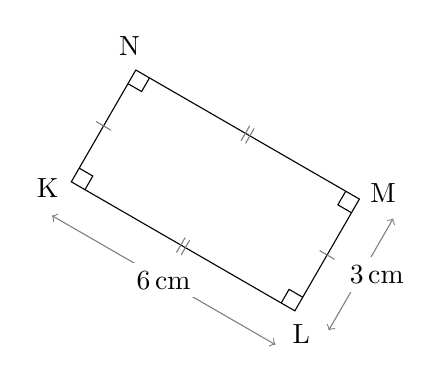
\begin{tikzpicture}[scale=1.1, baseline=(current bounding box.north)]
    \begin{scope}[rotate=-30]
        % Draw square
        \draw (0,0) coordinate (K) --
              ++(2.98,0) coordinate (L) --
              ++(0,1.49) coordinate (M) --
              ++(-2.98,0) coordinate (N) -- cycle;

        % Right angle markers
        \foreach \p/\q/\r in {N/K/L,K/L/M,L/M/N,M/N/K} {
            \pic [draw, -, angle radius=0.2cm] {right angle=\p--\q--\r};
        }

        % Vertex LABELS
        % Labels relative to shape geometry
        \node at ($(K)+(-0.2,-0.2)$) {K};
        \node at ($(L)+(0.2,-0.2)$) {L};
        \node at ($(M)+(0.2,0.2)$) {M};
        \node at ($(N)+(-0.2,0.2)$) {N};

        % double Tick marks across horizontal side K--L
        \draw[thin, gray]
            ($(K)!0.5!(L) + (-0.03,-0.10)$) --
            ($(K)!0.5!(L) + (-0.03,0.10)$);

        \draw[thin, gray]
            ($(K)!0.5!(L) + (0.03,-0.10)$) --
            ($(K)!0.5!(L) + (0.03,0.10)$);

        % double Tick marks across horizontal side N--M
        \draw[thin, gray]
            ($(N)!0.5!(M) + (-0.03,-0.10)$) --
            ($(N)!0.5!(M) + (-0.03,0.10)$);

        \draw[thin, gray]
            ($(N)!0.5!(M) + (0.03,-0.10)$) --
            ($(N)!0.5!(M) + (0.03,0.10)$);


        % Tick marks across vertical sides
        \draw[thin, gray]
            ($(L)!0.5!(M) + (-0.10,0)$) --
            ($(L)!0.5!(M) + (0.10,0)$);

        \draw[thin, gray]
            ($(K)!0.5!(N) + (-0.10,0)$) --
            ($(K)!0.5!(N) + (0.10,0)$);


        % dotted/dashed arrows shifted away from edges
        % Horizontal side (A-B), shifted down
        \draw[<->, gray]
            ($(K) + (0,-0.45cm)$) -- ($(L) + (0,-0.45cm)$)
            node[black, midway, fill=white, inner sep=3pt] {6\,cm};

        % Vertical side (B-C), shifted right
        \draw[<->, gray]
            ($(L) + (0.45cm,0)$) -- ($(M) + (0.45cm,0)$)
            node[black, midway, fill=white, xshift=2mm, inner sep=3pt] {3\,cm};

    \end{scope}
\end{tikzpicture}
\end{minipage}%
\hfill
\begin{minipage}{.4\textwidth}
  \begin{align*}
  \text{Area} &= lw \\
  \text{Area} &= \dotuline{~~~~~~~} \,\text{cm} \times \dotuline{~~~~~~~} \,\text{cm} \\
  \text{Area} &= \dotuline{~~~~~~~} \,\text{cm}^2
  \end{align*}
\end{minipage}

\end{document}
